\chapter{Introduction}

\label{chapter:intro}

Micro unmanned aerial vehicles (MAVs) recently saw a rise in usage across various fields. Drones are already wide used in cinematography \cite{Mademlis2020}, advertising \cite{Ullah2021} and in farming \cite{Kim2019}. 
City emergency departments use UAVs - firefighters can use them to see and evaluate the situation from the sky, localize the source of fire and put it out \cite{Pritzl2021}.
Another ffield where UAV's can be used in nearest future is transportastion. 
Fast parcel delivery \cite{San2018} and content transportastions \cite{Gupta2021,Aloqaily2022} are quite promissing fields of UAV application together with smart city comncept evolving \cite{Ortiz2019}.
Nowedays, even a collaborative transportation systems are not something fictional - swarms become more popular and that alows use them for a transportation of really huge objects \cite{Bacelar2020} that one drone can not lift. 
UAV's and MAV's are also wide used in the military industry\cite{Duz2021}.

As drones are used so widely, they should become more safe. 
UAV's are expensive and quite heavy, so accidents with them can cost a lot of money and somebody's lives. 
Even if a drone is on a remote controll, FOV of a pilot can not be bigger than FOV of his eyes (which is about $130^\circ$), but dangerous obsacles can appear from any side.
In this sence, autonomus robots can see and avoid obstacles much beter, but only if they have a well-designed system running onboard and enough sensors to cover the area around a drone.

Here where safety systems become important: if the only obstacles in the sky are birds, which usually are afraid of a noise from UAV, in a closed environment, in a forest or a city there can be much more hidrances: trees, humans, other UAV's, falling or flying objects, furniture etc.
UAV's can have many sensors pointing to all directins to make itself safe, and usually they are not used in some closed envieronments due to it's size.
For MAV's its size and weight can be obstructive, but they usually are used in a closed envieronment - they are small.
So it's always a tradeoff - the bigger UAV is the more there may be sensors on it, and the bigger should be surrending to use it. 

That is why a compact obstacle avoidance system is a very perspective field for research. 
Even though the idea is old, neither DJI, MRS, nor other research groups have a well-developed visual obstacle avoidance system. 
The best, for now, can be the Skydio system \footnotetext{\href{https://www.skydio.com/skydio-autonomy}{https://www.skydio.com/skydio-autonomy - Skydio autonomy}}, but their approach is for a forward-moving drones.

The inspiration for this project was taken from DJI obstacle avoidance technology introduced with the release of the DJI Mavic 3 drone\footnote{\href{https://www.dji.com/cz/mavic-3}{https://www.dji.com/cz/mavic-3 - DJI Mavic 3}}. 
It uses visual data from monocular cameras with overlapping sones to cover almost whole area around the UAV and react in a real-time on obstacles nearby. 
Unfortunately they have no publications or implementation details, so it's only a conclusion from publicly available information.

\section{Related Works}
There are several obstacle avoidance sensors used by various MAVs: stereo vision \cite{Ruf2018}, depth cameras (as Intel RealSense), monocular vision \cite{Mejias2010}, lidar (2d or 3d) \cite{Ramasamy2016}, sonar (ultrasonic), time of flight sensors, also combinations of them can be used. 
In \cite{Rambabu2015} the sensor fusion of ultrasonic and infrared sensors is presented.

Each of them has its pros and cons. 
3D lidars are more expensive than other sensors, but their efficiency is one of the best nowadays; 2d lidars are successfully used for ground vehicles, but they are not so suitable for most tasks for MAVs because a car can be modelled as a 2DoF system, while MAVs always have 6DoF. 
Depth cameras are more expensive than simple cameras. Ultrasonic and infrared sensors have distance limits and other minor issues ( a.e. sonar can be influenced by noise from the MAVs). 

In most articles stereo pair of two parallel cameras looking in the same direction is used (classical stereo pair) \cite{Yu2018, Lin2021, Xiao2019}, deep learning approaches \cite{Back2020, FragaLamas2019, Park2020, Roghair2021} and Convolutional Neural Networks \cite{Yu2013, Ma2020}. 
The real-time multi-camera feedback control system is introduced in \cite{He2021}, but this solution does not imply one drone, only multi-drone systems.

Real-time simultaneous localization and mapping (SLAM) systems can also be used for obstacle avoidance \cite{Moreno2014}. 
These problems are pretty closely related. 
SLAM keeps track of an object's position while constructing and updating a map of an unknown environment; obstacle avoidance is a problem of detecting and avoiding the nearest obstacles in an unknown environment to keep drones safe.
So both problems are related to making a 3D map of an unknown environment, but for obstacle avoidance, the precision of distance measurements to the nearest objects is much more critical.

Structure from Motion (SfM) is another possible algorithm that can be used to implement a system for avoiding obstacles. 
SfM is a method of depth map reconstruction from a set of explicit images, so using this approach, dense point clouds can be computed, and obstacles can be detected \cite{Lee2008}. 

\section{Problem definition}
\begin{figure}[t]
    \centering
    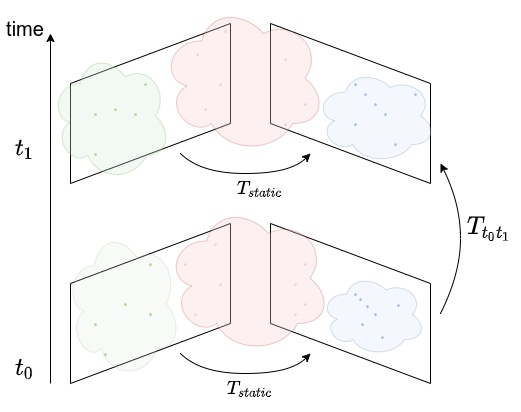
\includegraphics[width=0.7\textwidth]{graphics/general_scheme.png}
    \caption{General system scheme}
    \label{fig:intro_general}
\end{figure}

This thesis aims to design a visual obstacle avoidance system for MAVs, 3D model it, assemble a device, and measure its efficiency. 
A working solution assumes a MAV with limited size and lifting force, that limits number of sensors on it; onboard setup of two calibrated (\autoref{sec:prelimin_calibration}) cameras with known transformation between them.
Both cameras FOV have an overlapping zone big enough to detect close obstacles.
Cameras framerate guarantee system working in a real-time (at least 30fps), and images from all cameras are syncronised in time.
Computational power is enough to make a system real-time.
MAV flies in an envieroment whith some number of objects as an office or a room, to ensure that there is a sufficient number of features on images in a cameras' overlapping sone for a feature detecotor, and it should calculate the distance to all sorrounding objects with an allowable error.

On a figure \autoref{fig:intro_general} there is a scheme of a proposed system: $T_{static}$ is a transformation between cameras obtained after stereopair calibration. 
At each timestamp, new pair of images received.
Feature detector extract interesting points from the image, then all points in a \textit{red} zone are filtered and matched.
It can be done because they are from an overlapping zone. 
In such a way some 3d points are obtained already on a timestamp $t_0$. 
Then at a timestamp $t_1$ new pair of images arrives - and same process is repeated. 
Obtained pointcloud can be used further to fix the scale of a blue/green pointclouds obtained from SfM and see distance to objects that are not inside the overlaping zone.
Red pointcloud from $t_1$ also can be a starting point to use Iterative Closest Point algorithm to align red and blue points, because red has common points from both of them.